\documentclass[margin=8mm]{standalone}
\usepackage[T1]{fontenc}
\usepackage[utf8]{inputenc}
\usepackage{pgf,tikz}
\usepackage{utfsym}

\newcommand{\wall}[2]{% height, width in the plane
  \draw[fill, black] (0, 0) rectangle (#2, #1);}

\newcommand{\wheel}{%
  \draw[fill, black!60] (-3mm, -1mm) rectangle (3mm, 1mm); }

\newcommand{\robot}{%
  \node[anchor=center,circle, draw, inner sep=2.5mm] at (0,0) {};
  \begin{scope}[xshift=2mm, yshift=7mm]
    \wheel
  \end{scope}
  \begin{scope}[xshift=2mm, yshift=-7mm]
    \wheel
  \end{scope}
  \node[anchor=center, circle, inner sep=0.5mm, black!60,fill] at (-6mm, 0) {};
  %\draw[->, red!60!black] (0,0) to (20mm, 0);
  %\node at (20mm, 4mm) {$v$};
  %\draw[->, red!60!black] (0, 2.7mm) arc[radius=2.7mm, start angle=90, end angle=270];
  %\node at (-3mm, -1mm) {$\omega$};
}

\def\wthickness{0.2}

\begin{document}

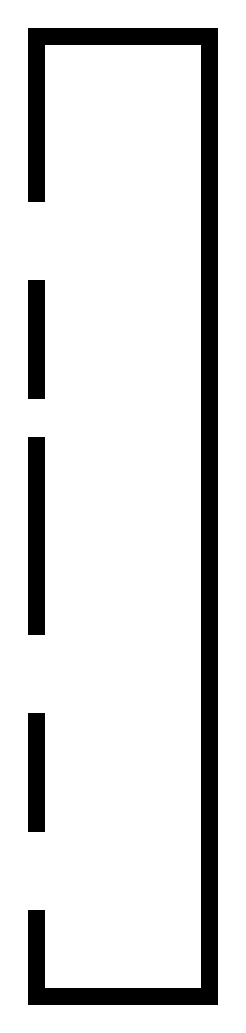
\begin{tikzpicture}[scale = 1]

  %\draw[fill, orange!20!white] (-2, -6)  rectangle (2,6);
  %\draw[step=1cm, blue!20!white, very thin] (-2, -6) grid (2,6);

  %\draw[->] (0,0) to (1cm, 0);
  %\draw[->] (0,0) to (0, 1cm);

  %%%%%%%%%%%%%%%%%%%%%%%%%%%%%%%%%%%%%%%%%%%%%%%%%%%%%%%%%
  % Outer walls
  %%%%%%%%%%%%%%%%%%%%%%%%%%%%%%%%%%%%%%%%%%%%%%%%%%%%%%%%%
  
  \begin{scope}[xshift=1cm, yshift=-6.2cm]
    \wall{12.4}{\wthickness}
  \end{scope}

  \begin{scope}[xshift=-1.2cm, yshift=-6.2cm]
    \wall{\wthickness}{2.2}
  \end{scope}
  \begin{scope}[xshift=-1.2cm, yshift=6cm]
    \wall{\wthickness}{2.2}
  \end{scope}

  
  %%%%%%%%%%%%%%%%%%%%%%%%%%%%%%%%%%%%%%%%%%%%%%%%%%%%%%%%%
  % Corridor
  %%%%%%%%%%%%%%%%%%%%%%%%%%%%%%%%%%%%%%%%%%%%%%%%%%%%%%%%%

  \begin{scope}[xshift=-1.2cm, yshift=-6.2cm]
    \wall{1.2}{\wthickness}
  \end{scope}
  \begin{scope}[xshift=-1.2cm, yshift=-4cm]
    \wall{1.5}{\wthickness}
  \end{scope}
  \begin{scope}[xshift=-1.2cm, yshift=-1.5cm]
    \wall{2.5}{\wthickness}
  \end{scope}
  \begin{scope}[xshift=-1.2cm, yshift=1.5cm]
    \wall{0.5}{\wthickness}
  \end{scope}
  \begin{scope}[xshift=-1.2cm, yshift=2cm]
    \wall{1.0}{\wthickness}
  \end{scope}
  \begin{scope}[xshift=-1.2cm, yshift=4cm]
    \wall{2}{\wthickness}
  \end{scope}


  %\begin{scope}[xshift=-4.5cm, yshift=-4cm, scale=0.5]
  %  \robot
  %\end{scope}

  %\node[circle, draw, inner sep=0.2mm, red!60!black, pin=20:{(3m, 3m)}] at (3,3) {Goal!};
  
\end{tikzpicture}
\end{document}
